\section{Two-stage Floquet preparation of a Bell-type BIC}
\label{sec:two_stage_protocol}

The effective Floquet description turns the static BIC condition into a
time-dependent control path. We exploit this observation to prepare the
Bell-type BIC from the absolute ground state in two coherent stages. The
state is propagated in the basis
\(\{|G\rangle,|1\rangle,|2\rangle,|k\rangle\}\), where
\(|G\rangle\equiv |g,g,0\rangle\),
\(|1\rangle\equiv |e,g,0\rangle\),
\(|2\rangle\equiv |g,e,0\rangle\), and
\(|k\rangle\equiv |g,g,1_k\rangle\). In the first stage, \(0<t<T_\pi\), a
local resonant drive is applied only to the first atom,
\begin{equation}
H_{\pi}(t)=\frac{\Omega_{\pi}(t)}{2}
\left[
e^{i\varphi_\pi}|1\rangle\langle G|
+ e^{-i\varphi_\pi}|G\rangle\langle 1|
\right],
\label{eq:local_pi_pulse}
\end{equation}
with a smooth pulse envelope
\begin{equation}
\Omega_{\pi}(t)=\frac{2\pi}{T_\pi}\sin^2\!\left(\frac{\pi t}{T_\pi}\right),
\qquad
\int_0^{T_\pi}\Omega_\pi(t)\,dt=\pi .
\label{eq:pi_pulse_envelope}
\end{equation}
The drive phase is chosen as \(\varphi_\pi=\pi/2\), which compensates the
phase acquired under a resonant \(\pi\)-pulse and prepares
\(|G\rangle\rightarrow |1\rangle\). During this loading step the Floquet
couplings are held at the initial dark-state values \(u_1=0\) and
\(u_2=u_0\), so that the prepared excitation is already aligned with the
initial dark atomic direction.

In the second stage, \(T_\pi<t<T_\pi+T\), the local loading pulse is switched
off and the Floquet modulation deforms the radiative couplings according to
\begin{equation}
u_1(\tau)=u_0\sin\theta(\tau),\qquad
u_2(\tau)=u_0\cos\theta(\tau),
\label{eq:floquet_coupling_path}
\end{equation}
where \(\tau=t-T_\pi\). We use the smooth quintic schedule
\begin{equation}
\theta(\tau)=\frac{\pi}{4}\left(10s^3-15s^4+6s^5\right),
\qquad s=\tau/T ,
\label{eq:quintic_schedule}
\end{equation}
which satisfies \(\dot{\theta}(0)=\dot{\theta}(T)=0\). For the symmetric
geometry considered here, the atomic component of the instantaneous dark
state follows
\begin{equation}
|D_a(\tau)\rangle =
\cos\theta(\tau)|e,g\rangle+\sin\theta(\tau)|g,e\rangle .
\label{eq:target_dark_atomic_path}
\end{equation}
Thus the protocol continuously maps the product excitation \(|e,g\rangle\)
onto the Bell state
\(|\Psi^+\rangle=(|e,g\rangle+|g,e\rangle)/\sqrt{2}\).

Finite-time errors are suppressed by adding the minimal counterdiabatic
correction in the atomic single-excitation subspace,
\begin{equation}
H_{\rm CD}(t)=\dot{\theta}(\tau)\sigma_y
= i\dot{\theta}(\tau)
\left(|2\rangle\langle 1|-|1\rangle\langle 2|\right).
\label{eq:atomic_cd_term}
\end{equation}
This term is not assumed to be the exact gauge potential of the fully dressed
BIC. Rather, it is used as a controlled benchmark that cancels the
nonadiabatic rotation error of the target atomic component. The full
finite-mode state obeys the effective central-sideband Schr\"odinger
equation,
\begin{align}
H_{\rm eff}(t)
&=
\sum_k \omega_k |k\rangle\langle k|
+\Omega_0\sum_{j=1,2}|j\rangle\langle j|
\nonumber\\
&\quad+
\sum_k\sum_{j=1,2}
\left[
u_j(t)g_{jk}|j\rangle\langle k|+\mathrm{H.c.}
\right]
+H_{\pi}(t)+H_{\rm CD}(t),
\label{eq:two_stage_effective_hamiltonian}
\end{align}
where \(H_\pi(t)=0\) during the Floquet passage and \(H_{\rm CD}(t)=0\) during
the loading step.

\begin{figure*}[t]
\centering
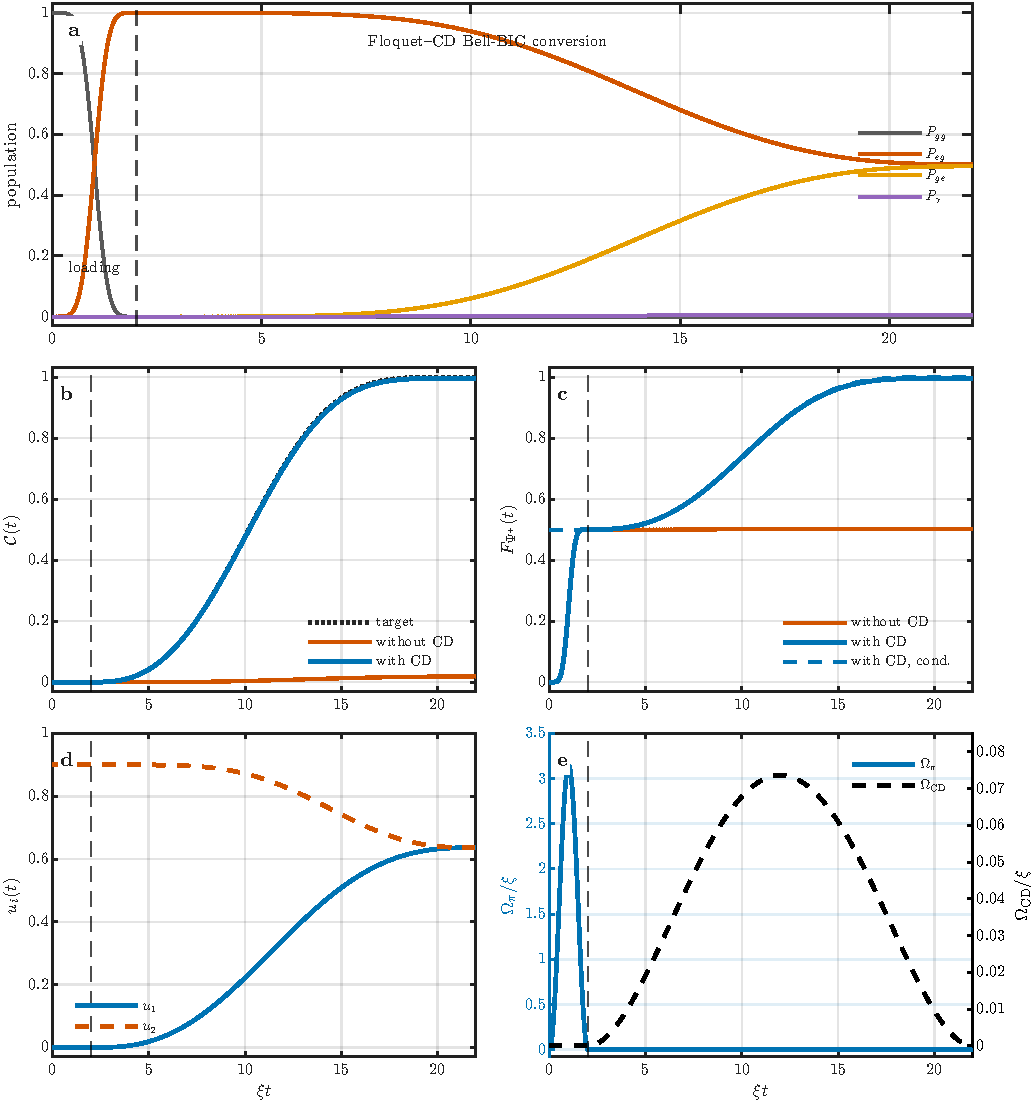
\includegraphics[width=\textwidth]{figures/Figure_TwoStage_Bell_BIC.pdf}
\caption{\textbf{Two-stage Floquet preparation of a Bell-type BIC.}
\textbf{a,} Population dynamics in a single coherent protocol. A local
\(\pi\)-pulse first loads the excitation into \(|e,g\rangle\); the
Floquet--counterdiabatic passage then converts the excitation into an equal
superposition of \(|e,g\rangle\) and \(|g,e\rangle\), while keeping the
photonic population small. \textbf{b,} Concurrence generated during the
protocol. Without the counterdiabatic term the state does not follow the
target path, whereas the CD-assisted protocol follows the ideal concurrence
curve. \textbf{c,} Bell-state fidelity
\(F_{\Psi^+}=|\langle\Psi^+|\psi(t)\rangle|^2\), together with the
conditional atomic fidelity. \textbf{d,} Floquet-renormalized couplings
\(u_1(t)\) and \(u_2(t)\). \textbf{e,} Local loading pulse
\(\Omega_\pi(t)\) and counterdiabatic amplitude \(\Omega_{\rm CD}(t)\).
The dashed vertical line marks the end of the loading stage.}
\label{fig:two_stage_bell_bic}
\end{figure*}

Figure~\ref{fig:two_stage_bell_bic} shows the complete preparation sequence.
For \(N_c=2004\), \(\xi T_\pi=2\), \(\xi T=20\), \(u_0=0.9\), and
\(\nu/\xi=8\), the loading pulse prepares the single-excitation product state
with \(P_{eg}(T_\pi)=0.99999999999990\). In the absence of the
counterdiabatic correction, the final concurrence remains small. By contrast,
the CD-assisted protocol reaches a final concurrence
\(\mathcal{C}=0.9959\), an unconditional Bell fidelity
\(F_{\Psi^+}=0.9959\), and a conditional atomic Bell fidelity
\(F_{\Psi^+}^{(a)}=0.99999\). The result demonstrates that the Floquet
couplings provide a direct control route from a locally prepared excitation
to the Bell component of a BIC, while the CD term converts this route into a
high-fidelity finite-time protocol.
